\subsection{Условие Брегга-Вульфа}
\begin{figure}[ht]
    \centering
    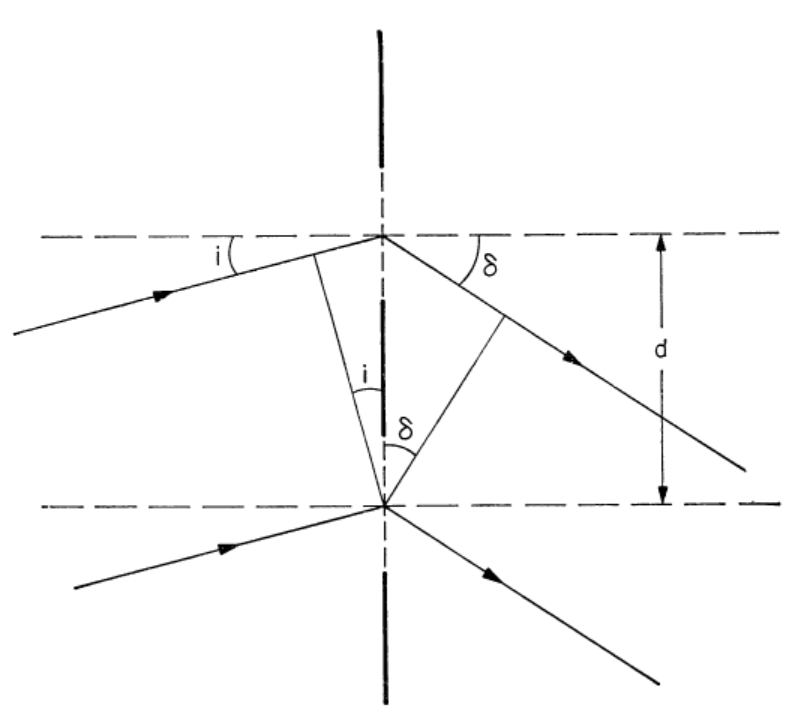
\includegraphics[width=0.4\textwidth]{figures/10_add_reshetka.png}
    \hspace{5 mm} 
    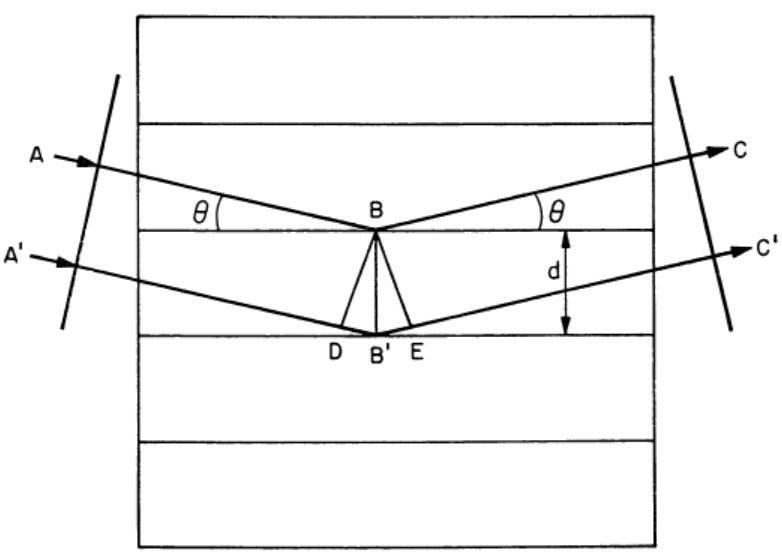
\includegraphics[width=0.4\textwidth]{figures/10_add_bregg.png}
    \caption{К формуле решетки плоской и объёмной}
    \label{fig:10_add}
\end{figure}

Помним формулу решетки, смотрим на левый рисунок(\ref{fig:10_add}), 
\begin{equation*}{}
	d (\sin i + \sin \delta) = \lambda,
\end{equation*}
 где ограничимся рассмотрением максимума первого порядка. 
Теперь рассмотрим правый рисунок(\ref{fig:10_add}) с объемной решеткой в разрезе.
Здесь аналогично интенсивность максимальна в том направлении, в котором волны складываются симфазно.

На рисунке $DB' + B'E = 2 d \sin \theta$, что с условием максимума даёт на закон Брегга-Вульфа:
\begin{equation*}
	2 d \sin \theta = m \lambda.
\end{equation*}
Таким образом получаем более жесткое условие на наблюдение $m$-го максимума дифракции.
Для объёмной решетки выбор угла падения определяет и длину волны и угол дифракции. 

Рассмотренная схема была впервые получена Бреггом и независимо от него Вульфом для ренгеновских лучей.
Напомним, что рентгеновский диапазон составляет от $10^{-3}$ нм до $100$ нм.
\textit{Жестким}  называют излучение с $\lambda < 0.2$ нм, оно обладает большой проникающей способностью в вещество.

Рассмотренная схема справа на рисунке(\ref{fig:10_add}) аналогична и по выводу для дифракции рентгеновских. Где уже нарисованные уровни, от которых происходит отражение -- \textit{атомные плоскости}, то есть плоскости в кристалле содержащее большое число атомов, до которых доходит рентгеновское излучение.
Отраженные же волны от кристалла рассматриваем так же, как отражение от разных атомных плоскостей.

Стоит заметит, что помимо максимумов, задаваемых условиям Брегга-Вульфа, есть ещё максимумы -- результаты отражения от разных слоев. Наиболее сильное отражение происходит от того слоя, где атомов больше.

Вдаваясь ещё в частности. Для монокристалла нужное найти положение в пространстве, при котором условие Брегга-Вульфа будет выполняться. В случае поликристалла и монохроматичного излучения найдется много кристаликов (плоскостей) для которых выполнится наше условие. На наборе таких плоскостей строится метод Дебая-Шеррера по изучению кристаллов в рентгеновском спектре.